% 问题二
\section{问题二的模型建立与求解}

\subsection{模型准备}

\subsubsection{数据来源与整合}

本问使用附件 1–4：品类日销量 $Q_{c,t}$、品类加权售价 $P_{c,t}$ 与批发价 $W_{c,t}$ 在附件 2、3 基础上沿用问题一的清洗与聚合口径构建（退货以负销量并入净销量），损耗率 $L_c$ 由附件 4 单品损耗率按固定销量份额加权聚合。

\subsubsection{统计口径}

关键量的统计口径如表 \ref{tab:q2_stats} 所示。

\begin{table}[htbp]
\centering
\caption{问题二统计口径}
\label{tab:q2_stats}
\begin{tabular}{cll}
\toprule
量 & 口径 & 来源 \\
\midrule
$Q_{c,t}$ 品类日净销量 & 附件 2 按单品—品类映射聚合，退货以负销量并入当日净销量 & 附件 2 \\
$W_{c,t}$ 品类批发价 & 附件 3 单品批发价按固定基期销量份额加权 & 附件 3 \\
$L_c$ 品类损耗率 & 附件 4 单品损耗率按固定销量份额加权：$L_c=\sum_i w_i L_i$（百分数，代入公式前除以 100） & 附件 4 \\
$P_{c,t}$ 品类售价 & 单品售价按\textbf{固定基期销量权重}加权（Laspeyres 型价格指数） & 附件 2 \\
\bottomrule
\end{tabular}
\end{table}

\subsection{模型建立}
\label{sec:q2_model}

\subsubsection{需求—价格关系：品类 Log-Log 弹性回归}

对品类 $c$ 建立双对数（常弹性）回归：
\begin{equation}
\ln Q_{c,t}=\alpha_c+\beta_c\ln P_{c,t}+\delta_c\,t+\sum_{k=1}^{6}\delta_{c,k}\,\mathbb{1}_{\{\mathrm{weekday}=k\}}+\sum_{m=1}^{11}\eta_{c,m}\,\mathbb{1}_{\{\mathrm{month}=m\}}+\varepsilon_{c,t},
\end{equation}
其中 $\beta_c$ 为价格弹性（预期为负），$t$ 为线性趋势项（防止伪回归），星期虚拟变量（基准周一）与月份虚拟变量（基准 1 月）刻画周期结构，$\delta_{c,k}$、$\eta_{c,m}$ 分别为星期与月份虚拟变量系数，记号与问题一残差回归（$\delta_k$、$\eta_m$）一致。双对数形式的优点在于弹性为常数，可直接外推“销量—价格”反事实，是销量—价格实证研究的标准形式 \cite{tellis1988}。

每个品类独立做 OLS 估计，报告弹性 $\hat\beta_c$、$t$ 值（显著性）、$R^2$ 与样本量，并做残差平稳性（DW/ADF）检验防止伪回归 \cite{wooldridge2010}。内生性处理上，价格与当期需求同时决定，OLS 可能有偏，稳健性做法是用滞后一期价格 $\ln P_{c,t-1}$ 替代当期价格重新估计，或采用工具变量，论文报告两种估计的差异作为稳健性证据 \cite{wooldridge2010}。销量截断方面，缺货日的销量低估真实需求，若缺货与价格相关（如低价日需求更高、更易缺货），弹性估计会受截断影响，作为局限写入小结。

价格口径与加价率的衔接：由于售价 $P=(1+k)W$，在控制批发价 $\ln W$ 后，$\ln(1+k)$ 的系数即 $\beta_c$，即“批发价不变时，加价率弹性等于价格弹性”，故 $\beta_c$ 同时刻画“销售总量对成本加成加价率”的敏感程度；反事实示例需注明“批发价不变”。

\subsubsection{最优定价：成本加成加价率解析解}

\textbf{有效进货成本}。损耗率 $L_c$ 表示进货量中最终损耗的比例，售出 1 kg 需进货 $1/(1-L_c)$ kg，故单位售出成本为 \cite{nahmias1982,blackburn2009,tang2018}
\begin{equation}
c'_{c,t}=\frac{W_{c,t}}{1-L_c}.
\end{equation}
注意附件 4 的损耗率为百分数（如 12.83 表示 12.83\%），代入上式前需除以 100，否则有效成本为负、临界比越界。

\textbf{常弹性最优加价率}。在参考点 $(\bar Q_c,\bar P_c)$ 处把需求近似为常弹性函数 $Q(P)=\bar Q_c(P/\bar P_c)^{\beta_c}$，单日利润为 \cite{petruzzi1999}
\begin{equation}
\pi(P)=\left(P-c'_{c,t}\right)\bar Q_c\left(\frac{P}{\bar P_c}\right)^{\beta_c}.
\end{equation}
对 $P$ 求导并令导数为零（记 $E_c=|\beta_c|>1$ 时为极大值）：
\begin{equation}
\frac{d\pi}{dP}=\bar Q_c\left(\frac{P}{\bar P_c}\right)^{\beta_c}\left[1+\beta_c\frac{P-c'_{c,t}}{P}\right]=0 \quad\Longrightarrow\quad P^*_{c,t}=\frac{E_c}{E_c-1}\,c'_{c,t}=\frac{E_c}{E_c-1}\cdot\frac{W_{c,t}}{1-L_c}.
\end{equation}
对应批发价加价率（即“成本加成”倍率）为
\begin{equation}
m^*_c=\frac{P^*_{c,t}}{W_{c,t}}-1=\frac{E_c}{(E_c-1)(1-L_c)}-1.
\end{equation}
该式等价于垄断定价的逆弹性规则（Lerner 条件）$(P^*-c')/P^*=1/E_c$ \cite{mascolel1995}，且解析最优价处报童临界比恰为 $\kappa^*=(P^*-c')/P^*=1/E_c$，与 \ref{sec:newsvendor} 节衔接。

需说明：$\kappa^*=1/E_c$ 仅在解析最优解处成立；本问各品类弹性均小于 1、落入数值求解分支（\ref{sec:result}节），临界比一律按定义 $\kappa=(P^*-c')/P^*$ 直接计算（表 \ref{tab:q2_pricing}），不直接使用该关系。

\textbf{关键性质与决策规则}：$m^*_c$ 只依赖弹性与损耗率、与批发价 $W_{c,t}$ 无关。因此商超可在凌晨未知当日批发价时预先确定品类加价率策略，到货后按实际批发价确定售价 $P^*_{c,t}=(1+m^*_c)W_{c,t}$——这既对应题面“成本加成定价”，也化解了“凌晨 3:00–4:00 不知具体进货价”的时序约束。

\textbf{边界处理与数值求解}：

\begin{enumerate}
\item 若历史估计 $E_c\le 1$（无弹性或弱弹性），解析解不存在或无最大值，改在历史加价率百分位区间 $[m_{5\%},m_{95\%}]$ 内以 201 点等距网格数值搜索最优加价率 \cite{tellis1988}；
\item 网格搜索中利润一律按\textbf{截断后的最终售价} $P=\min(\max((1+k)W,P_5),P_{95})$ 评估，需求仍以最终售价为自变量，避免“评估价与最终售价脱节”；
\item 解析解分支同样将最优价截断在历史价格区间 $[P_5,P_{95}]$ 内，防止常弹性外推越界；
\item 输出中标注各品类弹性 $E_c$、加价率 $m^*_c$ 及是否命中解析解，保证可追溯。
\end{enumerate}

\textbf{说明}：当 $E_c<1$ 时利润函数在可行加价率区间内单调递增，网格最优落在可行域边界——多数品类为加价率上界 $m_{95\%}$，花菜类与水生根茎类受价格上界 $P_{95}$ 约束（见9.1节）；论文中的最优加价率应理解为“\textbf{历史交易区间约束下的最优}”，而非无条件全局最优，区间边界敏感性见 \ref{sensitivity_analysis} 节。

\subsubsection{基准需求预测：去价格序列 + 趋势—周期外推}

\textbf{去价格变换}。先用第 \ref{sec:q2_model} 节估计的弹性 $\hat\beta_c$ 把历史销量折算到统一参考价 $\bar P_c$（取历史加权均价）下的“无价格效应需求”：
\begin{equation}
Q^0_{c,t}=Q_{c,t}\left(\frac{\bar P_c}{P_{c,t}}\right)^{\hat\beta_c}.
\end{equation}
因 $\hat\beta_c<0$，历史价高于参考价的日子需求被上调、低于参考价的日子被下调，序列 $Q^0$ 保留趋势/星期/季节结构但剔除价格影响。\textbf{若不先剔除价格效应就直接预测原始销量、再乘价格比，价格效应会被重复计入} \cite{taylor2018,hyndman2018}。

\textbf{外推预测}。对去价格序列 $Q^0_{c,t}$ 建模并外推未来一周参考价下的基准需求 $\bar Q_{c,t}$ 与残差标准差 $\sigma_{c,t}$（模型设计以 Prophet 为基准，含周与年季节项；代码实现为等价的含线性趋势、星期与月份虚拟变量的回归外推，并对数均值修正，即 $\bar Q=\exp(\widehat{\ln Q}+\mathrm{MSE}/2)$、$\sigma=\bar Q\sqrt{\exp(\mathrm{MSE})-1}$，两种实现等价 \cite{taylor2018,hyndman2018}）。

\textbf{最优定价下的需求分布（乘性缩放）}。在最优售价 $P^*$ 下，需求按弹性整体缩放（乘性需求假设，是定价—报童联合问题的标准设定 \cite{petruzzi1999}）：
\begin{equation}
\mu_{c,t}(P^*)=\bar Q_{c,t}\left(\frac{P^*_{c,t}}{\bar P_c}\right)^{\hat\beta_c},\qquad \sigma_{c,t}(P^*)=\sigma_{c,t}\left(\frac{P^*_{c,t}}{\bar P_c}\right)^{\hat\beta_c}.
\end{equation}
假设含义：价格只改变需求水平、不改变变异系数，分布形态随价格同比例缩放；该假设已在模型假设中说明。

\subsubsection{报童补货模型}
\label{sec:newsvendor}

设进货可售量 $y=(1-L_c)R$，需求分布为 $F$（均值为 $\mu$、标准差为 $\sigma$、价格为 $P^*$），单位售出成本 $c'=W/(1-L_c)$，残值为 0。报童模型的最优条件对任意需求分布成立 \cite{silver2016,khouja1999,petruzzi1999}：
\begin{equation}
E\pi=P^*\cdot E[\min(D,y)]-c'\cdot y.
\end{equation}
最优可售量满足分位数条件 $F(y^*)=\kappa_{c,t}$，临界比为
\begin{equation}
\kappa_{c,t}=\frac{P^*_{c,t}-c'_{c,t}}{P^*_{c,t}}=\frac{P^*_{c,t}-W_{c,t}/(1-L_c)}{P^*_{c,t}}.
\end{equation}

\textbf{分布口径与问题一衔接}：问题一按 AIC 为各品类从伽马、对数正态两类右偏连续分布中选择拟合（花叶类、花菜类、水生根茎类、茄类为伽马，辣椒类、食用菌为对数正态）。为与代码实现一致，本问统一采用对数正态矩匹配分位数作为实现口径：由预测期均值 $\mu$ 与标准差 $\sigma$ 矩匹配对数参数（$\mu_{\ln}=\ln\left(\mu^2/\sqrt{\mu^2+\sigma^2}\right)$、$\sigma_{\ln}=\sqrt{\ln\left(1+\sigma^2/\mu^2\right)}$）后计算 $y^*=\exp\left(\mu_{\ln}+\sigma_{\ln}\,\Phi^{-1}(\kappa)\right)$，伽马与对数正态分位数之差并入近似误差。
\begin{equation}
y^*_{c,t}=\mu_{c,t}(P^*)+\sigma_{c,t}(P^*)\,z_c(\kappa_{c,t}),
\end{equation}
其中 $z_c(\kappa)=F_c^{-1}(\kappa)$ 为品类 $c$ 拟合分布标准化后的 $\kappa$ 分位数；不依赖参数分布时，用历史残差的经验分位数 $\hat F^{-1}(\kappa)$ 替代 \cite{agrawal1996}。每日品类补货总量为
\begin{equation}
R_{c,t}=\frac{y^*_{c,t}}{1-L_c}=\frac{\mu_{c,t}(P^*)+\sigma_{c,t}(P^*)\,z_c(\kappa_{c,t})}{1-L_c}.
\end{equation}

说明：
\begin{itemize}
\item 正态分布只是 $z_c(\kappa)=\Phi^{-1}(\kappa)$ 的特例；右偏分布下同一 $\kappa$ 的分位数与正态明显不同（如 $\kappa=0.5$ 时正态给均值、lognormal 给中位数），故统一采用对数正态矩匹配分位数，正态仅作近似对比 \cite{agrawal1996}；
\item $z_c(\kappa)<0$ 表示“负安全库存”，即可售量 $y^*$ 低于需求均值 $\mu(P^*)$。对右偏分布均值高于中位数，$z_c(\kappa)<0$ 的临界 $\kappa$ 大于 0.5；本问 6 品类临界比均小于 0.5，均处于“负安全库存”区域——需求波动大且超量损耗成本高时，以适度缺货风险换取更低的超量损耗成本，属报童最优条件的正常结果；
\item 除以 $(1-L_c)$ 是把可售量折算回进货量，补偿损耗 \cite{nahmias1982}；
\item 口径局限：问题一拟合的是已售销量而非真实需求，缺货日销量低估需求，报童补货量可能系统性偏低。
\end{itemize}

确定性对照：忽略需求波动（$z_c=0$）时的补货量为 $R^0_{c,t}=\mu_{c,t}(P^*)/(1-L_c)$，作为“无安全库存”基准。

\subsubsection{品类独立优化的合理性：相关性只进入方差、不进期望}

问题一识别出品类销量存在协同变动，本节论证逐品类独立定价与补货不损失期望利润。记品类 $c$ 的期望利润 $f_c(R_c)=E_{D_c}\left[\pi_c(R_c;D_c)\right]$，其只依赖品类 $c$ 自身的边际需求分布 $F_c$（$\pi_c$ 中不含其他品类的销量或价格）。

\textbf{命题 1（期望可加与可分最大化）}：期望的线性性给出 $E[\sum_c\pi_c]=\sum_c E[\pi_c]$；又因每个 $f_c$ 只含自己的决策 $R_c$ 且可行集可分，最大化的“和”可逐项分解：
\begin{equation}
\max_{R\in X}\sum_{c=1}^{6}f_c(R_c)=\sum_{c=1}^{6}\max_{R_c\in X_c}f_c(R_c).
\end{equation}
该分解性是多品无约束报童问题的标准结论：无容量约束时，多品报童退化为相互独立的单品问题 \cite{silver2016}。

\textbf{命题 2（最优订货只依赖边际分布）}：报童最优条件 $F_c(y^*_c)=\kappa_c$ 只含品类 $c$ 的边际 CDF。品类间相关性刻画的是联合分布结构，不改变任何一个边际分布 $F_c$，故不改变任一品类的最优订货量 $y^*_c$ 与补货量 $R^*_c$（单周期报童模型的基本性质 \cite{khouja1999,petruzzi1999}）。

\textbf{推论}：在风险中性假设下（题面“收益最大”即指最大化期望利润），逐品类独立优化与整体联合优化的最优决策相同。协方差矩阵既不进入临界比条件（\ref{sec:newsvendor}节），也不进入最优价公式（\ref{sec:q2_model}节），最优补货量与最优售价均与品类间相关性无关；相关性只进入总利润的方差分解：
\begin{equation}
\mathrm{Var}\left(\sum_c\pi_c\right)=\sum_c\mathrm{Var}(\pi_c)+2\sum_{c<c'}\mathrm{Cov}(\pi_c,\pi_{c'}).
\end{equation}
正相关通过协方差项放大总利润波动，但不改变期望利润（组合理论的基本结论 \cite{markowitz1952}）。

\textbf{结论成立的三项条件}：
\begin{enumerate}
\item 目标可加：各品类利润函数互不包含（本模型需求函数无交叉价格项）；
\item 决策集可分：无共享资金、货架或订货容量约束（问题二成立，问题三不成立）；
\item 边际分布外生：品类 $c$ 的需求边际分布不受其他品类定价决策的影响。
\end{enumerate}

\textbf{失效情形与本文定位}：若商超风险厌恶或存在联合风险约束（资金预算、亏损概率上限），利润联动会改变最优决策 \cite{chen2009}；存在共享容量约束，需联合优化 \cite{abdelmalek2004}；需求存在替代/互补（涨价导致跨品类转移），独立定价不是真实意义上的全局最优。其中 ③ 最贴近本题现实：问题一的相关性分析只能识别“销量同步变动”，不能识别因果替代结构，交叉价格弹性建模留待问题四的数据扩展；本文在 \ref{stability_q2} 节用交叉价格弹性联合定价模拟作为稳健性对照。


\subsection{模型求解与结果分析}
\label{sec:result}

\subsubsection{弹性估计结果}

对 6 个品类分别估计 Log-Log 回归，结果如表 \ref{tab:q2_elasticity} 所示（样本期 1095 天，$n$ 为各品类正销量日样本量；参考价为历史加权均价，参考需求为正销量日均值）。

\begin{table}[htbp]
\centering
\caption{品类价格弹性与定价参数}
\label{tab:q2_elasticity}
\begin{tabular}{lccccccccccc}
\toprule
品类 & 价格弹性 $\hat\beta_c$ & $t$ 值 & $R^2$ & 样本量 $n$ & 参考价 $\bar P_c$（元/kg） & 参考需求 $\bar Q_c$（kg） & 有效成本 $c'$（元/kg） & 加价率 $m_{5\%}$ & 加价率 $m_{95\%}$ & 最优加价率 $m^*_c$ & 是否解析解 \\
\midrule
花叶类 & -0.45 & -6.79 & 0.40 & 1085 & 5.89 & 183.22 & 4.11 & 0.44 & 1.01 & 1.01 & 否 \\
花菜类 & -0.50 & -5.45 & 0.31 & 1084 & 9.95 & 38.57 & 9.69 & 0.27 & 0.79 & 0.71 & 否 \\
水生根茎类 & -0.07 & -0.70 & 0.61 & 1085 & 9.22 & 37.45 & 12.93 & 0.26 & 0.70 & 0.44 & 否 \\
茄类 & -0.26 & -3.16 & 0.52 & 1050 & 8.80 & 21.38 & 4.41 & 0.30 & 0.90 & 0.90 & 否 \\
辣椒类 & -0.13 & -3.03 & 0.45 & 1085 & 8.63 & 84.52 & 3.49 & 0.26 & 1.14 & 1.14 & 否 \\
食用菌 & -0.31 & -5.28 & 0.41 & 1085 & 11.09 & 70.21 & 2.76 & 0.35 & 0.82 & 0.82 & 否 \\
\bottomrule
\end{tabular}
\end{table}

解读如下：

\begin{itemize}
\item 全部品类的价格弹性均为负，其中花叶类（-0.45）、花菜类（-0.50）需求价格敏感度最高，水生根茎类（-0.07）几乎无价格弹性；除水生根茎类（$t=-0.70$，不显著）外，其余品类弹性均在 1\% 水平显著；
\item 由于“批发价不变时加价率弹性等于价格弹性”（\ref{sec:q2_model}节），表 \ref{tab:q2_elasticity} 的 $\hat\beta_c$ 即销售总量对成本加成加价率的敏感度：花叶类加价率每提高 1\%，销量约下降 0.45\%；
\item \textbf{所有品类 $E_c=|\beta_c|<1$，均不满足解析解条件}，表 \ref{tab:q2_elasticity} 的最优加价率均为“历史加价率区间 $[m_{5\%},m_{95\%}]$ 网格 201 点的数值最优”，即历史区间约束下的最优，而非无条件解析最优；
\item 水生根茎类弹性不显著，其定价结论的证据强度相应降低，加价率主要由历史区间约束决定，需谨慎解读。
\end{itemize}

\begin{figure}[htbp]
\centering

\includegraphics[width=0.9\textwidth]{../figures/q2_elasticity_fit.pdf}
\caption{品类需求—价格弹性拟合（散点为去日历效应后的 $\ln$ 销量与 $\ln$ 价格，红色直线为弹性拟合线，标注 $\beta$、$t$ 与 $R^2$）}
\label{fig:q2_elasticity}
\end{figure}
由图 \ref{fig:q2_elasticity} 可见，各品类需求—价格散点整体呈负向倾斜，其中水生根茎类斜率较平缓（对应弹性 -0.07）；各面板标注的 $\beta$、$t$、$R^2$ 与表 \ref{tab:q2_elasticity} 一一对应，水生根茎类拟合线接近水平、散点分散，直观反映其弹性不显著。
\subsubsection{最优定价策略}

基于表 \ref{tab:q2_elasticity} 的弹性与加价率，代入最近一周批发价后得到未来一周固定的定价策略，如表 \ref{tab:q2_pricing} 所示（批发价取 2023-06-24 至 06-30 最近均价；参考价 $\bar P_c$ 为历史加权均价，供 \ref{sec:q2_model} 节乘性缩放 $P^*/\bar P_c$ 对照；加价率与临界比在周内保持不变）。
\begin{table}[H]
\centering
\caption{品类最优定价策略（未来一周）}
\label{tab:q2_pricing}
\begin{tabular}{lccccc}
\toprule
品类 & 批发价 $W$（元/kg） & 参考价 $\bar P_c$（元/kg） & 最优售价 $P^*$（元/kg） & 加价率 $m^*$ & 临界比 $\kappa$ \\
\midrule
花叶类 & 3.59 & 5.89 & 7.22 & 1.01 & 0.43 \\
花菜类 & 8.19 & 9.95 & 14.00 & 0.71 & 0.31 \\
水生根茎类 & 11.16 & 9.22 & 16.07 & 0.44 & 0.20 \\
茄类 & 4.11 & 8.80 & 7.81 & 0.90 & 0.44 \\
辣椒类 & 3.17 & 8.63 & 6.79 & 1.14 & 0.49 \\
食用菌 & 2.50 & 11.09 & 4.53 & 0.82 & 0.39 \\
\bottomrule
\end{tabular}
\end{table}

由 $\frac{d\pi}{dP}=\bar Q_c\left(P/\bar P_c\right)^{\beta_c}\left(1-E_c+E_c\,c'/P\right)$ 可见，当 $E_c=|\beta_c|<1$（需求缺乏价格弹性）时该导数对一切可行售价恒为正（因 $1-E_c>0$ 且 $E_c\,c'/P>0$），价格上调的收入增量超过销量缩减造成的损失，利润函数在可行域内随价格单调上升，最优加价率落在可行域边界：花叶类、茄类、辣椒类、食用菌的加价率取到历史加价率上界 $m_{95\%}$；花菜类与水生根茎类的最优售价被约束在历史价格区间上界 $P_{95}$（分别为 14.00 元/kg 与 16.07 元/kg）。因此该策略的稳健解读是“在历史交易区间内使期望利润最大化的加价率”，而非无条件全局最优；区间边界敏感性见 \ref{sensitivity_analysis} 节。

\begin{figure}[H]
\centering

\includegraphics[width=0.9\textwidth]{../figures/q2_price_curve.pdf}
\caption{期望利润—售价曲线（蓝色阴影为历史价格 $P_5$–$P_{95}$ 区间，红色虚线为最优售价 $P^*$）}
\label{fig:q2_price_curve}
\end{figure}

图 \ref{fig:q2_price_curve} 展示了各品类的期望利润—售价曲线：利润随售价上升并在区间边界达到峰值，红色虚线标出表 \ref{tab:q2_pricing} 的最优售价，与数值搜索结果一致。需注意，常弹性函数形式只在参考点附近可信：若脱离历史价格区间向外推，需求在远高价区可能转为强弹性而出现新的峰值，故本文不宣称无条件全局最优。

\subsubsection{需求预测与报童补货}

先按 \ref{sec:q2_model} 节在参考价下外推未来 7 天基准需求，再按最优售价做乘性缩放并代入报童模型，得到每日补货量与期望利润。

\begin{table}[H]
\centering
\caption{未来 7 天参考价下基准需求（中间输入，均值 $\pm$ 标准差，kg）}
\label{tab:q2_forecast_input}
\begin{tabular}{lccccccc}
\toprule
品类 & 07-01 & 07-02 & 07-03 & 07-04 & 07-05 & 07-06 & 07-07 \\
\midrule
花叶类 & 232.74 $\pm$ 84.74 & 223.95 $\pm$ 81.54 & 164.15 $\pm$ 59.76 & 159.99 $\pm$ 58.25 & 163.99 $\pm$ 59.71 & 160.14 $\pm$ 58.31 & 174.50 $\pm$ 63.53 \\
花菜类 & 37.96 $\pm$ 21.84 & 35.94 $\pm$ 20.68 & 24.57 $\pm$ 14.14 & 25.18 $\pm$ 14.49 & 25.03 $\pm$ 14.40 & 24.54 $\pm$ 14.12 & 28.27 $\pm$ 16.27 \\
水生根茎类 & 59.19 $\pm$ 35.83 & 54.36 $\pm$ 32.90 & 35.45 $\pm$ 21.46 & 35.90 $\pm$ 21.73 & 34.86 $\pm$ 21.10 & 34.61 $\pm$ 20.95 & 43.64 $\pm$ 26.42 \\
茄类 & 30.93 $\pm$ 15.06 & 29.78 $\pm$ 14.50 & 22.47 $\pm$ 10.94 & 20.76 $\pm$ 10.11 & 20.82 $\pm$ 10.14 & 21.33 $\pm$ 10.39 & 24.22 $\pm$ 11.80 \\
辣椒类 & 97.44 $\pm$ 41.05 & 92.44 $\pm$ 38.94 & 66.66 $\pm$ 28.08 & 64.74 $\pm$ 27.27 & 65.61 $\pm$ 27.64 & 65.30 $\pm$ 27.51 & 72.01 $\pm$ 30.34 \\
食用菌 & 69.58 $\pm$ 35.20 & 65.99 $\pm$ 33.38 & 43.93 $\pm$ 22.22 & 42.21 $\pm$ 21.35 & 46.54 $\pm$ 23.54 & 44.90 $\pm$ 22.71 & 53.05 $\pm$ 26.83 \\
\bottomrule
\end{tabular}
\end{table}

\begin{table}[H]
\centering
\caption{未来 7 天每日补货总量 $R_{c,t}$（kg）}
\label{tab:q2_replenishment}
\begin{tabular}{lcccccccc}
\toprule
品类 & 07-01 & 07-02 & 07-03 & 07-04 & 07-05 & 07-06 & 07-07 & 7 天合计 \\
\midrule
花叶类 & 215.13 & 207.00 & 151.72 & 147.88 & 151.58 & 148.02 & 161.29 & 1182.61 \\
花菜类 & 25.07 & 23.74 & 16.23 & 16.63 & 16.53 & 16.20 & 18.67 & 133.07 \\
水生根茎类 & 34.94 & 32.09 & 20.93 & 21.19 & 20.57 & 20.43 & 25.76 & 175.91 \\
茄类 & 28.51 & 27.45 & 20.71 & 19.14 & 19.20 & 19.66 & 22.33 & 157.01 \\
辣椒类 & 100.50 & 95.34 & 68.75 & 66.77 & 67.66 & 67.35 & 74.27 & 540.64 \\
食用菌 & 79.55 & 75.44 & 50.22 & 48.26 & 53.21 & 51.33 & 60.65 & 418.66 \\
\midrule
合计 & 483.70 & 461.05 & 328.56 & 319.87 & 328.75 & 322.99 & 362.97 & 2607.89 \\
\bottomrule
\end{tabular}
\end{table}

\begin{figure}[H]
\centering
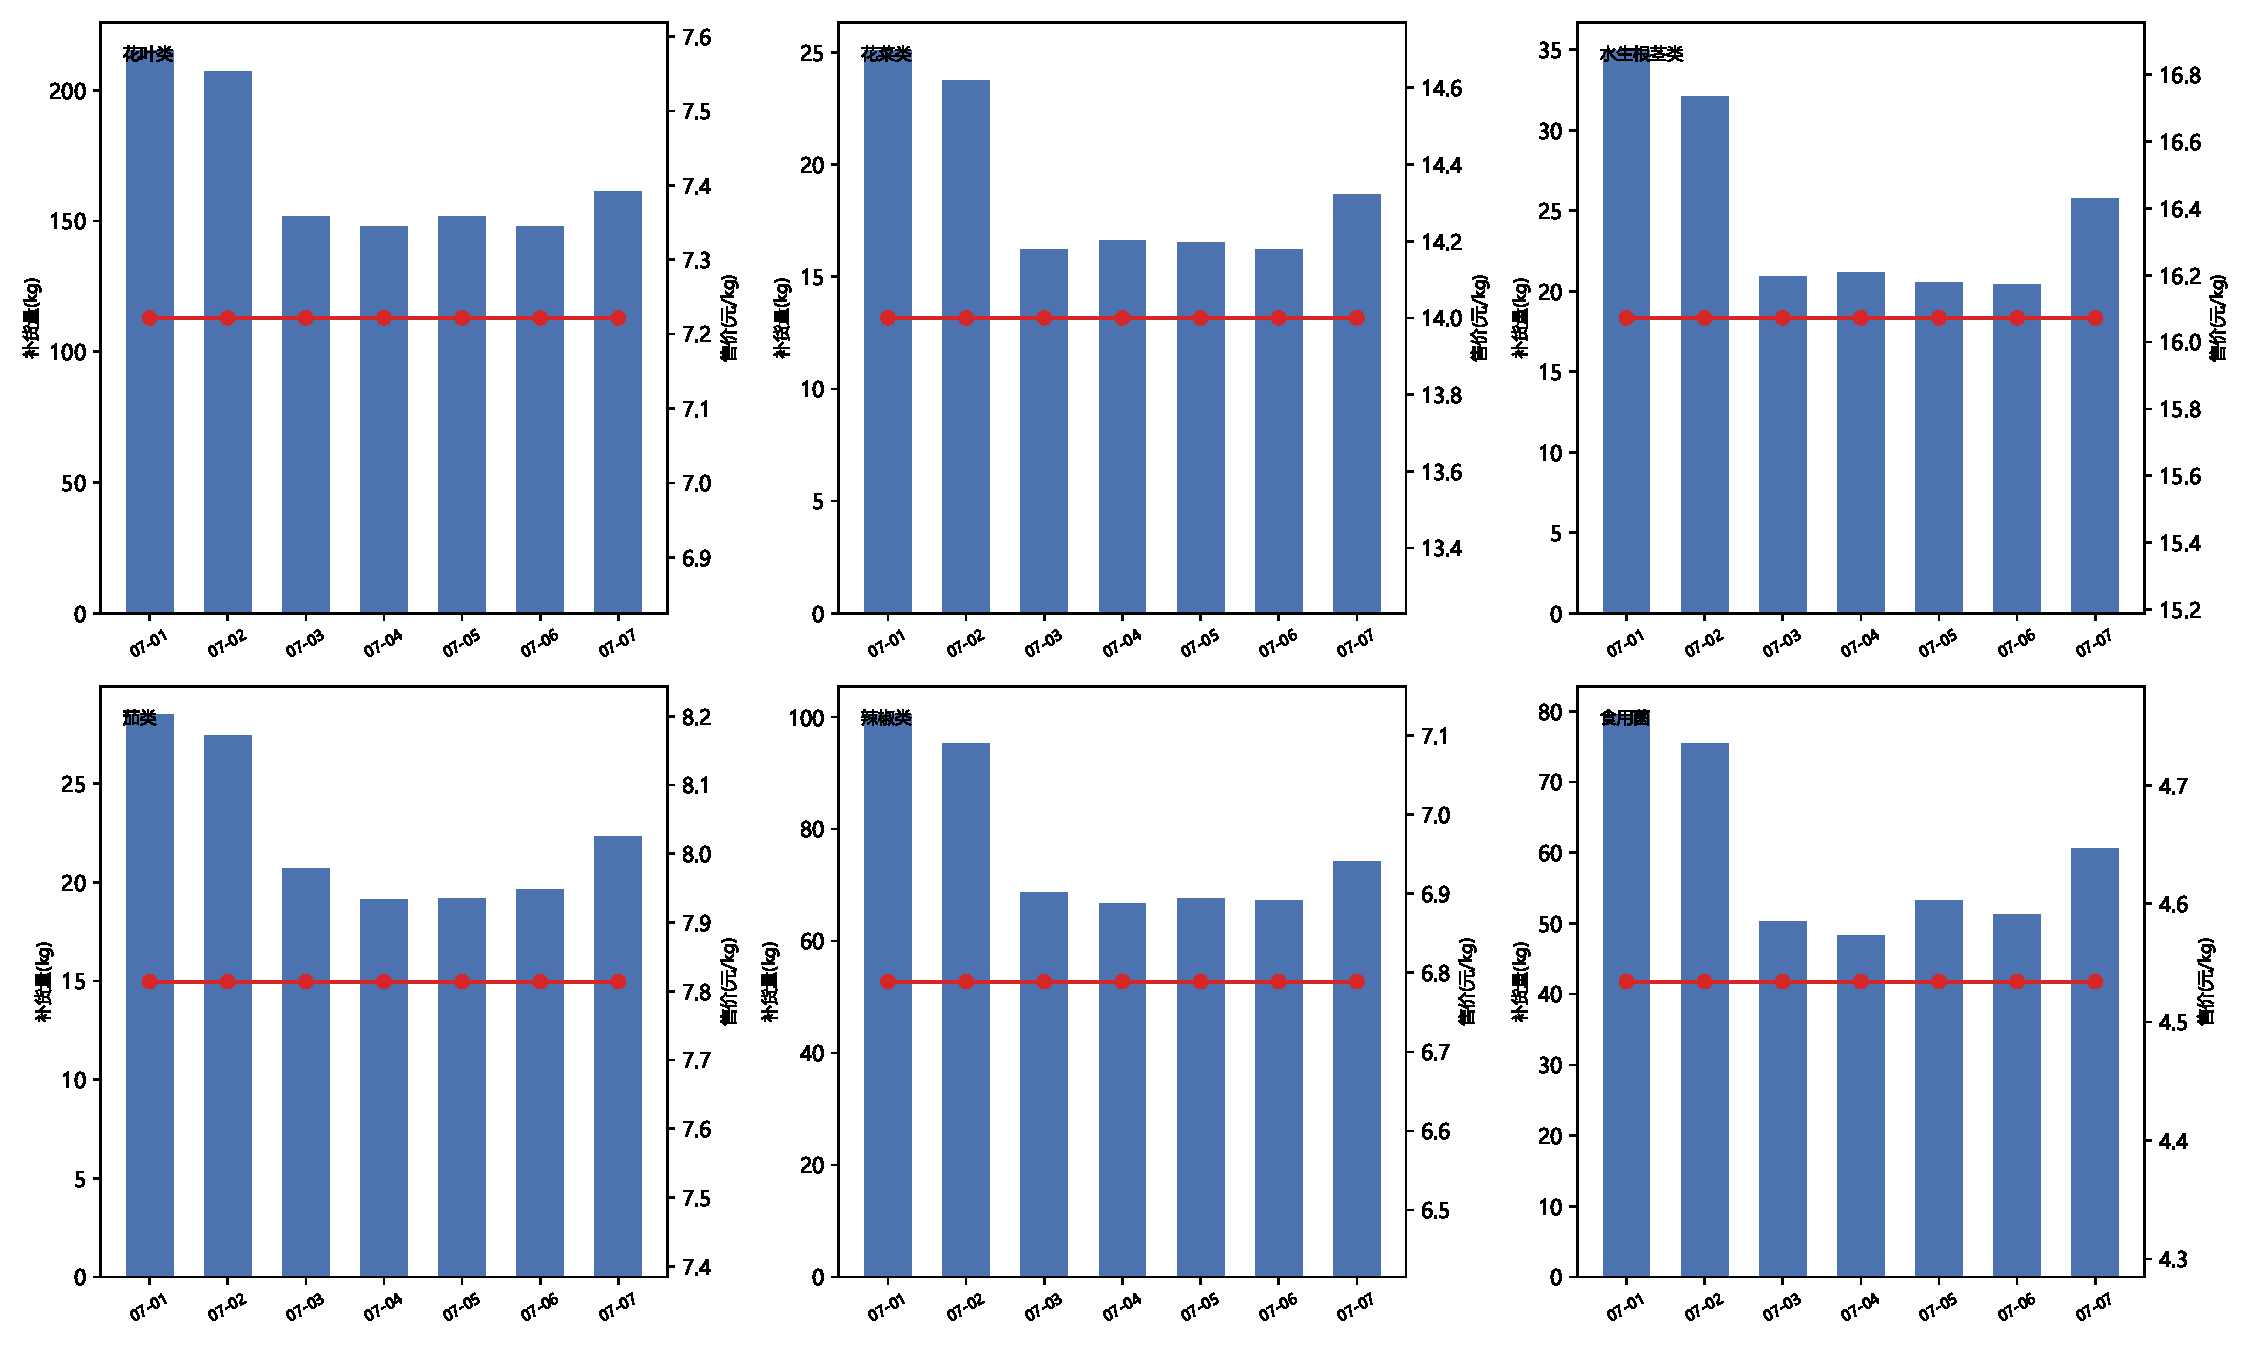
\includegraphics[width=0.8\textwidth]{../figures/q2_replenishment.pdf}
\caption{未来 7 天每日补货量（柱状图，左轴）与最优售价水平线（红色折线，右轴）}
\label{fig:q2_replenishment}
\end{figure}

图 \ref{fig:q2_replenishment} 直观展示各品类补货量随周内需求节奏波动，同时售价在整个预测期内保持恒定（加价率策略周内固定）。主要结果解读如下：

\begin{itemize}
\item \textbf{总量}：未来一周总补货量 2607.89 kg，总期望利润 5305.19 元；
\item \textbf{节奏}：补货量呈周末集中（7 月 1 日与 7 月 2 日合计 944.75 kg，占全周 36.2\%）、周中回落、周五小幅回升的周内结构，与表 \ref{tab:q2_forecast_input} 的“周末偏置”需求结构一致；
\item \textbf{花叶类}为最大补货品类（7 天合计 1182.61 kg，占总量 45.3\%），加价率 1.01、售价 7.22 元/kg，弹性 -0.45 意味着加价 1\% 仅损失约 0.45\% 销量，定价上调空间最大；
\item \textbf{水生根茎类}补货量（175.91 kg）明显低于确定性基准（332.03 kg）：其临界比 $\kappa=0.20$ 为各品类最小，安全库存为负（$z_c(\kappa)<0$），反映其在需求波动大、损耗成本高的条件下，以适度缺货风险换取更低的超量损耗成本；
\item \textbf{利润贡献}：花叶类（2517.33 元）与辣椒类（1209.04 元）合计占 7 天总期望利润的 70.2\%，构成利润的主要来源。
\end{itemize}

\subsubsection{决策时序与操作含义}

策略执行分三步：① 商超在 2023-06-30 依据表 \ref{tab:q2_elasticity} 的弹性与损耗率确定 6 个品类的加价率 $m^*_c$，周内保持不变（对应“加价率与批发价无关”的性质，见 \ref{sec:q2_model} 节）；② 每日凌晨批发价到货后按 $P^*=(1+m^*)W$ 确定实际售价（对应“凌晨未知当日进货价”的时序约束）；③ 按表 \ref{tab:q2_replenishment} 的每日补货量执行采购。批发价 $\pm10\%$ 的扰动风险由 \ref{sensitivity_analysis} 节灵敏度覆盖。


\subsection{小结}

问题二以“Log-Log 弹性回归 $\to$ 最优加价率 $\to$ 去价格预测 $\to$ 报童补货”四步完成品类级定价与补货决策。弹性回归表明，6 个品类需求价格弹性均为负，花叶类（-0.45）、花菜类（-0.50）弹性最强，水生根茎类（-0.07）弹性不显著；批发价不变时，价格弹性即销售总量对加价率的弹性。由于各品类 $|\beta_c|<1$，最优加价率为历史加价率区间约束下的数值解——花叶类加价率 1.01（售价 7.22 元/kg）、花菜类 0.71（14.00 元/kg）、水生根茎类 0.44（16.07 元/kg）、茄类 0.90（7.81 元/kg）、辣椒类 1.14（6.79 元/kg）、食用菌 0.82（4.53 元/kg），且与批发价无关、可提前确定。未来一周总补货量 2607.89 kg、总期望利润 5305.19 元，补货节奏与问题一周内周期一致，水生根茎类因需求波动大、临界比最小而明显减少补货量。独立性论证表明，风险中性下逐品类独立优化即可达到期望利润最优，相关性只进入总利润方差；后 28 天滚动回测 MAPE 20.6\%–37.2\%、差分进化多种子结果一致、联合定价模拟显示交叉价格效应仅对最优价格水平产生边际影响，主结论稳健。

\textbf{局限}：水生根茎类弹性不显著，其定价结论证据不足；缺货日销量截断使补货量可能系统性偏低；固定权重价格指数因品类单品进出而不连续；模型不含日内清仓与跨期需求转移，风险中性假设下未考虑资金预算等联合风险约束。